\chapter{NLMyo : Traitement de rapport textuel par LLMs}

\section{Contexte}
Les récentes avancées dans le \gls{nlp} ont permis de révolutionner la manière de traiter et d'exploiter les données sous forme de texte libre. \gls{impatient} utilise un système à base de règles et de correspondance exacte des mots pour analyser les comptes-rendus de biopsie. Cette approche présente des limites importantes en terme de flexibilité et de précision et demande l'établissement d'un vocabulaire normalisé au préalable. 

Récemment, la mise à disposition de \gls{llms} performants et accessibles ouvre la porte à la création d'outils plus performants et flexibles pour le traitement de ces comptes-rendus. Ces système basé sur une approche sémantique et multi-langues éliminent la nécessitée de définir un vocabulaire standard. Ansi nous avons développé \gls{nlmyo} (fig \ref{fig:nlmyo_logo}), une boite à outils basée sur les \gls{llms} mettant à disposition quatre outils généralistes pour le traitement de comptes-rendus médicaux: outil d'anonymisation, d'extraction d'information, de classification automatique et de création de moteur de recherche. L'ensemble de ces outils et des modèles utilisés est représenté dans la figure \ref{fig:nlmyo_struct}.
\begin{figure}[htbp]
 \centering
 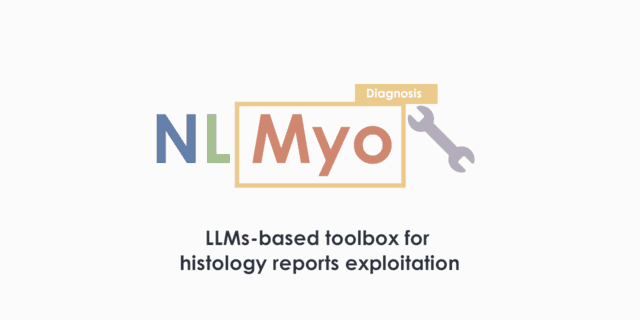
\includegraphics[width=0.5\textwidth]{figures/nlmyo_banner.png}
 \caption[Logo NLMyo]{Logo de NLMyo}
 \label{fig:nlmyo_logo}
\end{figure}
\begin{figure}[htbp]
 \centering
 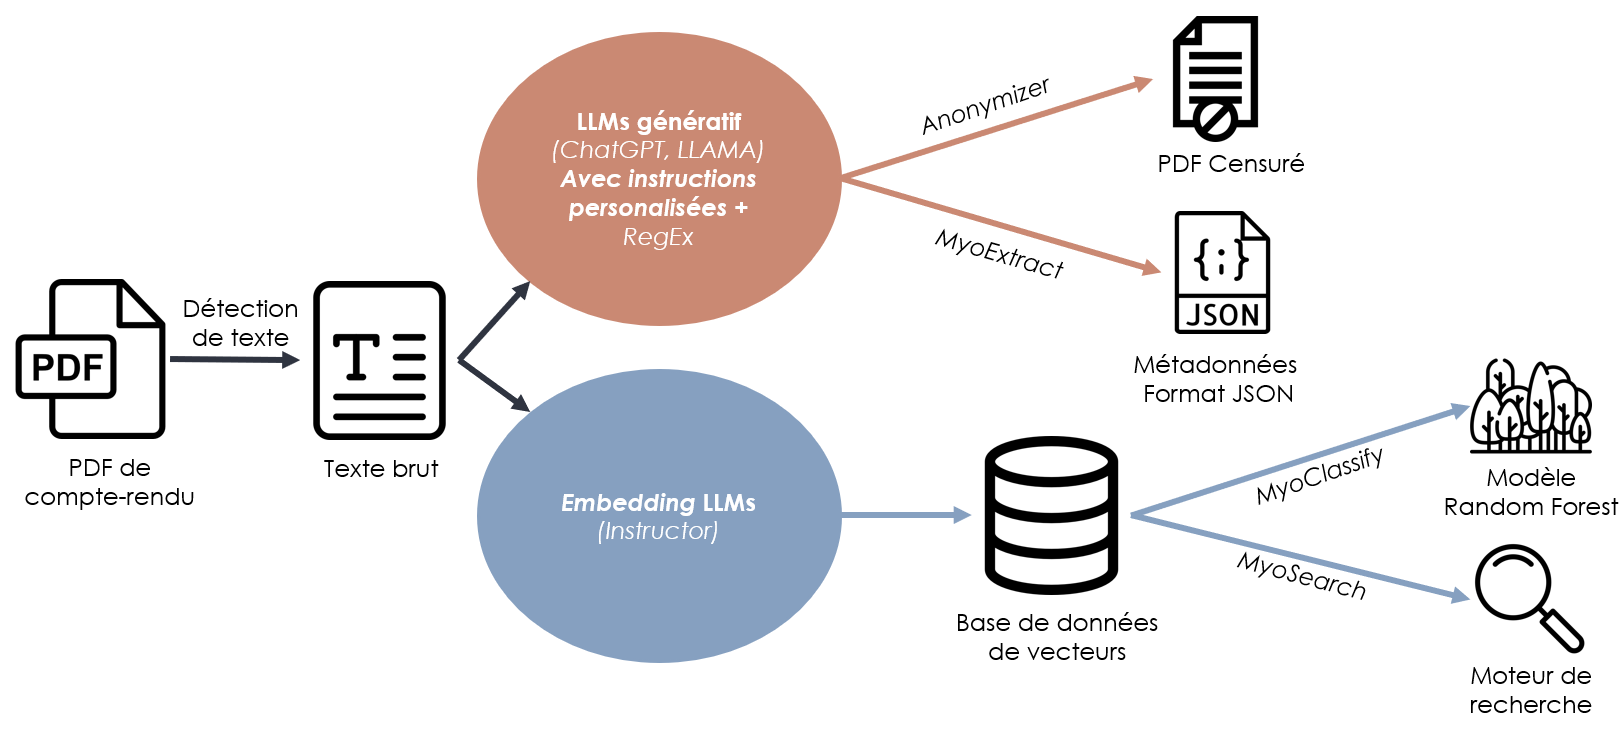
\includegraphics[width=1\textwidth]{figures/nlmyo_struct.png}
 \caption[Structure de NLMyo]{Structure de NLMyo}
 \label{fig:nlmyo_struct}
\end{figure}
\section{\textit{Anonymizer}: un outil d'anonymisation}
Le premier outil de \gls{nlmyo} est \textit{Anonymizer}, un outil permettant de supprimer automatiquement les informations identifiantes des comptes-rendus médicaux. Dans les comptes-rendus de biopsie de l'institut de myologie que nous traitons, deux données identifiantes et personnelles sont présentes et doivent être retirées: le nom du patient (et du personnel médical) ainsi que la date de naissance du patient. Non seulement ces informations ne sont pas utiles pour les analyses subséquentes mais de plus, par respect pour le \gls{rgpd} et la vie privée, ces informations ne doivent être accessibles qu'aux professionnels médicaux en charge du patient. L'anonymisation des rapports est donc une étape essentielle avant le transfert de ces données, leur numérisation et leur analyse.

Afin de traiter un grand volume de rapports et d'éliminer le travail manuel nécessaire, nous avons tenter d'automatiser la tache d'anonymisation via deux approches: un approche traditionnelle par\gls{regex} et une approche novatrice par\gls{llms}.

\subsection{Anonymisation par RegEx}
En première intention, nous avons développé une méthode basée sur les \gls{regex} pour leur simplicité à mettre en place et leur rapidité d'exécution (coûts en puissance de calcul faible). Le tableau \ref{tab:regex} liste les \gls{regex} utilisées pour capturer les informations de noms et de dates. Les comptes-rendus de biopsie sont semi-structurés. Pour la plupart le nom du patient est facilement identifiable car il est précédé par le préfixe: "Nom: ". Ceci est facilement capturable par la première \gls{regex} listée dans le tableau. Ensuite pour les autres cas de figure, comme les noms de famille sont souvent en majuscule et les prénom commencent souvent pas une majuscule, nous avons développé deux autres \gls{regex} pour capturer les couples de mots dont un est en majuscule et le second commence par une majuscule (ou inversement, ligne 2 et 3 du tableau). 
Ensuite, une troisième \gls{regex} a été ajoutée pour détecter les dates au format JJ-MM-AAAA ou JJ.MM.AAAA (ligne 3 du tableau). Finalement une dernière \gls{regex} est utilisée pour essayer de trouver le numéro de biopsie dans le document afin de renommer le fichier avec un nom unique et anonyme (ligne 4 du tableau). 
\begin{table}[htbp]
\centering
\caption{Expressions régulières pour extraire les noms et les dates}
\label{tab:regex}
\begin{tabular}{|l|l|l|}
\hline
\textbf{Expression régulière} & \textbf{Syntaxe} & \textbf{Exemples d'utilisation} \\ \hline
Nom patient & Nom.*: *([A-Za-zÀ-ÿ- ]+) & Nom : John Doe \\ \hline
Nom patient 2& (([A-Z][a-zÀ-ÿ-]\{3,\} ?)+ ([A-Z-]\{3,\} ?)+) & DOE John \\ \hline
Nom patient 3 & (([A-Z-]\{3,\} ?)+ ([A-Z][a-zÀ-ÿ-]\{3,\} ?)+) & John Joe DOE \\ \hline
Date & ([(.]?[0-9]\{1,2\}[./][0-9]\{1,2\}[./][0-9]\{1,4\}[().]?) & 01/01/2023, 02.02.2023 \\ \hline
N° Biopsie & ([0-9]\{3,8\}[-/]?[0-9]\{0,3\}) & 9876-54, 1234/56 \\ \hline
\end{tabular}
\end{table}
\begin{figure}[htbp]
 \centering
 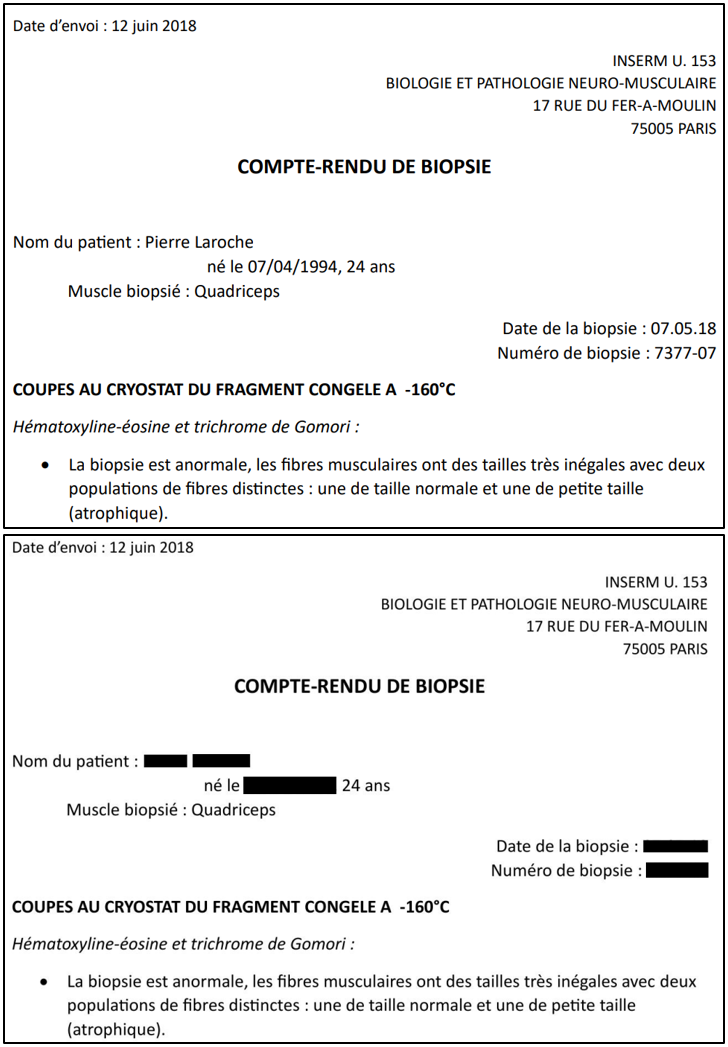
\includegraphics[width=1\textwidth]{figures/regex.png}
 \caption[Exemple anonymisation RegEx]{Exemple d'anonymisation d'un rapport de biopsie factice avec la méthode RegEx. En haut le rapport à l'état brut, en bas le rapport censuré.}
 \label{fig:regex}
\end{figure}

La figure \ref{fig:regex} présente les résultats de la technique d'anonymisation par \gls{regex} sur l'entête d'un rapport factice de patient mais avec une structure similaire aux rapport de l'institut de myologie de Paris. Les noms et les dates ont été censurés correctement et la méthode a produit de bon résultats. Cependant cette méthode est insuffisante car elle est peu sensible et spécifique. Le tableau \ref{tab:regex_fail} liste trois exemples de cas où cette méthode ne fonctionne pas et produit des erreurs. Il est possible de corriger ces erreurs en augmentant la somme de \gls{regex} utilisée, mais augmenter le nom de \gls{regex} augmente aussi potentiellement le nombre de faux positifs. De plus il n'est pas toujours possible de construire une \gls{regex} adaptée pour extraire une information précise. Nous avons alors exploré la capacité des \gls{llms} pour la recherche et l'extraction de ces informations de manière plus robuste et flexible que la méthode \gls{regex}.
\begin{table}[htbp]
\centering
\caption{Exemples de faux positifs ou faux négatifs de la méthode RegEx}
\label{tab:regex_fail}
\begin{tabularx}{\textwidth}{|X|X|X|X|}
\hline
\textbf{Texte} & \textbf{RegEx déclenchée} & \textbf{Type} & \textbf{Commentaire} \\ \hline
\textit{PAS Staining} & Nom patient 3 & Faux Positif & Nom de coloration dont la notation est confondue avec le motif "NOM Prénom" \\ \hline
\textit{Louis C. Dupont} & N/A & Faux Négatif & La présence du "C." au centre ne permet pas aux RegEx de nom de se déclencher \\ \hline
\textit{12 mars 2001} & N/A & Faux Négatif & La notation de date avec un mois en lettres ne permet pas à la RegEx de date de se déclencher \\ \hline
\textit{1996-04} & N° Biopsie & Faux Positif & La notation de date AAAA-MM déclenche la \gls{regex} de numéro de biopsie. \\ \hline
\end{tabularx}
\end{table}

\subsection{Anonymisation par LLMs}
Les \gls{llms} sont basés sur la compréhension du sens sémantique du texte là où les \gls{regex} sont basée sur le principe de motif de caractères et donc sur la structure du document. L'idée de l'anonymisation par \gls{llms} est d'utiliser un modèle génératif auquel on fournis une instruction et le texte à anonymiser. L'instruction fournie liste les informations à extraire du texte et spécifie le format de sortie. Pour intégrer ces modèles génératif à notre programme, nous voulons récupérer les informations extraites dans un format exploitable informatiquement, par exemple au format JSON. Le format JSON représente un dictionnaire qui est utilisable ensuite par l'application pour censurer les PDF à partir des informations extraites.

\subsection{Instruction personnalisée et \textit{one-shot learning}}
Nous avons construit une instruction personnalisée en 3 parties qui intègre une méthode de \textit{one-shot learning}. Les trois parties sont: (i) la description de la tâche à effectuer, (ii) un exemple de réalisation de la tâche \textit{(one-shot learning)}, (iii) le texte d'intérêt à anonymiser.
Voici un exemple d'instruction que nous utilisons pour réaliser l'extraction des noms et des dates dans les rapports:
\begin{quote}
Tu es un assistant qui extrait des informations d'un texte libre. Le format de ta réponse doit être un format JSON valide qui respecte le nom des clés founie. Si une valeur est manquante, indique simplement N/A, n'essaie pas d'inventer. Voici la liste des informations à récupérer, les clés JSON sont indiquées entre parenthèses : nom complet (name), dates (date).

ENTRÉE :

Kendrick Lamar et Jane Clinton sont asymptomatiques. Date de naissance : 16 février 1991, numéro de biopsie : 666-77. Ce rapport a été expédié le 01.04.1991.

SORTIE :

\{"name" :["Kendrick Lamar", "Jane Clinton"], "date" : ["16 février 1991", "01.04.1991"]\}

ENTRÉE :

<texte à analyser>

SORTIE :
\end{quote}

La partie précédant le mot clé "ENTREE" correspond à l'instruction décrivant précisément la tâche à réaliser au modèle (liste des informations à extraire, format de sortie et comportement attendu). Le premier couple "ENTREE" et "SORTIE" correspond à un exemple de réalisation de la tâche, ce qui permet de spécifier le schéma JSON attendu au modèle (\textit{one-shot learning}). Puis le second couple "ENTREE", "SORTIE" correspond à l'endroit où l'on injecte notre texte d'intérêt à analyser et spécifie au modèle que l'on attend maintenant une sortie textuel au format JSON pour l'entrée précédente.

\subsection{Exemple et comparaison à la méthode RegEx}
\begin{figure}[htbp]
 \centering
 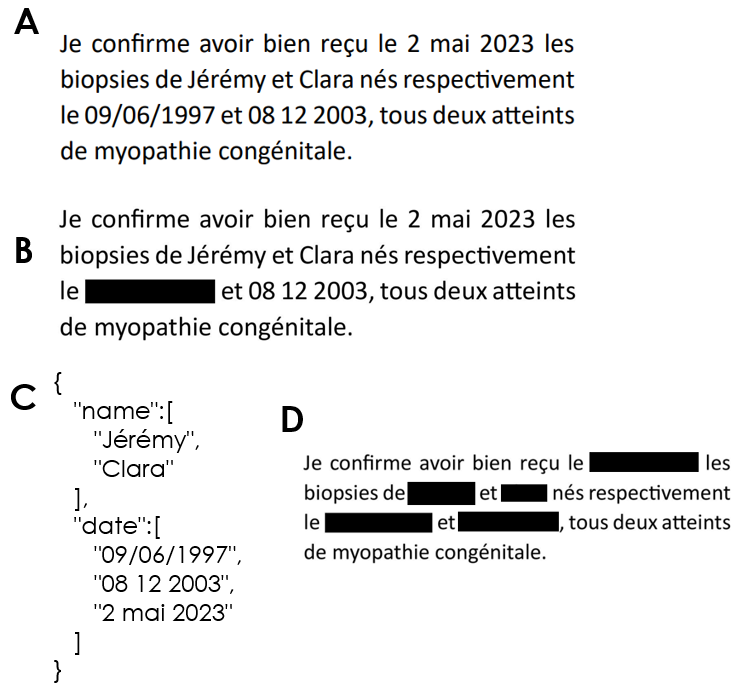
\includegraphics[width=0.8\textwidth]{figures/llms_anonym.png}
 \caption[Exemple anonymisation LLMs]{Exemple d'anonymisation d'un courrier médical factice avec la méthode par LLMs. (A) Texte brut, (B) Anonymisation par RegEx, (C) JSON brut généré par le \gls{llms} GPT-3.5-turbo (OpenAI), (D) Anonymisation à partir du JSON généré par \gls{llms}.}
 \label{fig:llms_anonym}
\end{figure}

Dans cet exemple (figure \ref{fig:llms_anonym}), nous avons construit un début de courrier médical factice faisant figurer des informations personnelles qui se sont pas détectable par notre méthode \gls{regex}. Les prénoms "Jérémy" et "Clara", ainsi que les dates "2 mai 2023" et "08 12 2003" n'ont pas été détectés par la méthodes \gls{regex} et n'ont pas été censurés. On observe par contre que la méthode par \gls{llms} (C et D) a été capable d'identifier ces informations et de les extraire du texte. Cet exemple montre que les \gls{llms} peuvent être la base d'un système d'anonymisation plus flexible et moins dépendant de la structure du document.

\section{\textit{MyoExtract}: un outil d'extraction d'information}
A partir des résultats encourageants obtenu la technique d'anonymisation par LLMs pour l'extraction d'information, nous avons voulu étendre le champs des informations extraites de manière automatique à partir de texte libre. Nous avons utilisé la même stratégie d'extraction d'information, c'est à dire l'utilisation de \gls{llms} génératifs mais avec une instruction légèrement différente. Cette fois-ci nous avons ajouté une liste plus importante d'informations à extraire non pas dans le but d'anonymiser le document, mais d'en extraire les méta-données. Par exemple nous avons chercher à extraire: les noms, date de naissance, date d'envoi de la biopsie, numéro de biopsie, muscle prélevé, diagnostic final. De plus nous avons chercher à savoir s'il était possible d'extraire s'il est mention d'anomalie pour certaines colorations tel que la coloration PAS, Soudan, COX, ATP et Phosphorilase. Cette extraction d'information pourrait permettre d'annoter automatiquement les rapports avec une liste d'anomalie détectée pour chaque coloration. De même que précédemment, nous avons construit une instruction personnalisée en 3 parties (description, exemple, texte à analyser.)

Voici un exemple d'instruction que nous utilisons pour réaliser l'extraction des méta-données et d'anomalies générales des colorations à partir de rapports:
\begin{quote}
Tu es un assistant qui extrait des informations d'un texte libre. Le format de ta réponse doit être un format JSON valide qui respecte le nom des clés founie. Si une valeur est manquante, indique simplement N/A, n'essaie pas d'inventer. Formate les dates sous la forme DD-MM-YYYY et convertis les âges en années (0 si inférieur à 1 an). Voici la liste des informations à récupérer, les clés JSON sont indiquées entre parenthèses : nom complet (name), âge (age), date de naissance (birth), date de la biopsie (biodate), date d'envoi de la biopsie (sending), muscle (muscle), numéro de la biopsie (bionumber), diagnostic (diag), présence d'une anomalie dans la coloration du PAS (PAS), présence d'une anomalie dans la coloration Soudan (Soudan), présence d'une anomalie dans la coloration COX (COX), présence d'une anomalie dans la coloration ATP (ATP), présence d'une anomalie dans la coloration Phosphorylase (phospho)

ENTRÉE:

Kendrick Lamar et Jane Clinton ne sont pas asymptomatique. Date de naissance: 16 février 1991, numéro de biopsie: 666-77. Anomalie forte à la coloration PAS mais pas d'anomalie à la coloration lipide soudan. Le tableau est révélateur d'une myopathie à némaline

SORTIE:

\{"name":["Kendrick Lamar", "Jane Clinton"], "age":"N/A", "birth": "16-02-1991", "biodate": "N/A"", "sending": "N/A"", "muscle": "N/A"", "bionumber": "666-77", "diag": "myopathie à némaline", "PAS": "yes", "Soudan": "no", "COX": "N/A", "ATP": "N/A", "phospho": "N/A"\}

ENTRÉE :

<texte à analyser>

SORTIE :
\end{quote}

\subsection{Exemple d'extraction d'information}
Pour cet exemple d'utilisation nous avons généré un rapport factice de patient avec une structure similaire aux rapports de l'institut de myologie de Paris qui reprend des observations typiques trouvées dans les rapports réel de biopsie. Ce rapport est disponible en figure \ref{fig:factice_report}. 
\begin{figure}[htbp]
 \centering
 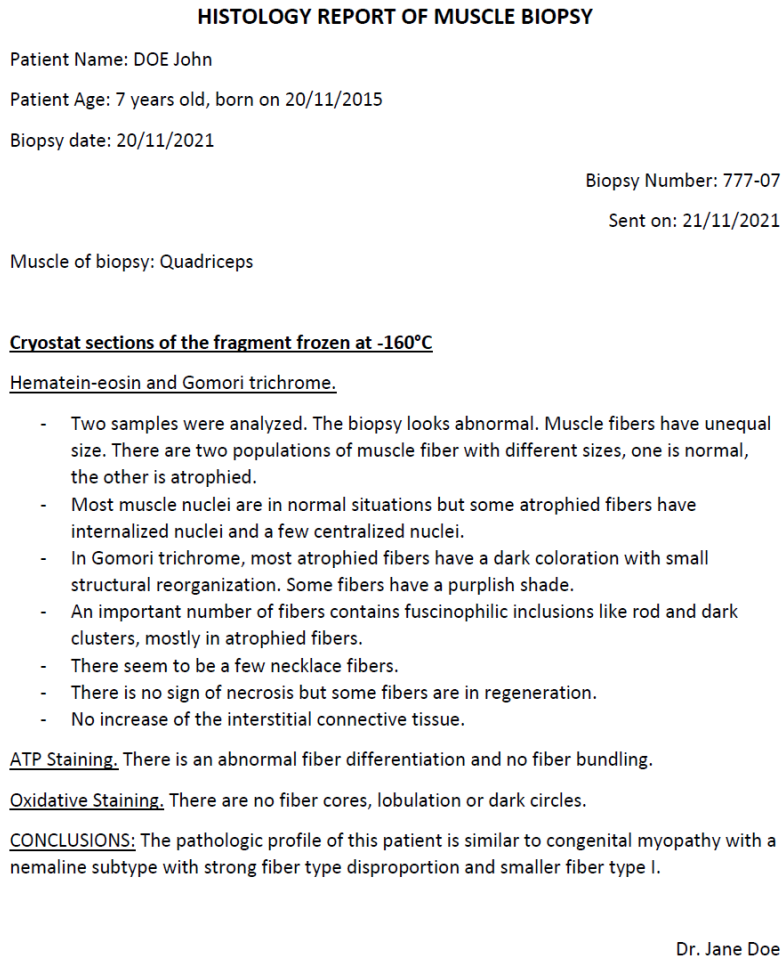
\includegraphics[width=1\textwidth]{figures/pdf_biopsie.png}
 \caption[Rapport de biopsie factice]{Exemple rapport de biopsie factice}
 \label{fig:factice_report}
\end{figure}

Les résultats de l'extraction d'information présentés dans le tableau \ref{tab:json_data} montrent que le modèle d'\textit{OpenAI} GPT-3.5-turbo est capable d'extraire l'ensemble des informations demandées de manière satisfaisante tout en étant capable de détecter l'absence de certaines informations. Concernant le modèle \textit{Vicuna-7B}, qui a l'avantage d'être auto-hébergé et donc d'être utilisable pour des données sensibles, les performances sont moindres. En effet, six données sur treize (diagnostic et anomalies) demandées sont tout simplement manquante dans le JSON de sortie. Cependant pour les sept données (nom, âge, dates, muscle et numéro de biopsie) présentes, les résultats sont satisfaisant, le modèle a extrait les bonne informations.

Il est important de noter qu'en terme de ressources de calcul et de temps de d'inférence, \textit{GPT-3.5} possède un avantage non-négligeable car ce modèle n'est accessible que par une \gls{api}. Les coûts de calcul pour l'application sont donc nul et la requête ne prend que quelques secondes à être réalisée. Pour \textit{Vicuna}, le modèle auto-hébergé, chaque requête requiert une quantité importante de ressources de calcul et monopolise ces ressources pour un temps important (environ 1min30 par document). Ces coûts en ressources et en temps de calcul couplé à une précision plus faible, rendent difficile l'exploitation de modèle \gls{llms} génératif auto-hébergé pour la tâche d'extraction d'informations à travers une interface en ligne.
\begin{table}[htbp]
\centering
\caption{Résultats de \textit{MyoExtract} pour \textit{GPT-3.5-turbo} and \textit{Vicuna7B}}
\label{tab:json_data}
\begin{tabularx}{\textwidth}{|X|X|X|}
\hline
\textbf{Information} & \textbf{GPT-3.5-turbo} & \textbf{Vicuna7B} \\ \hline
Nom & DOE John & DOE John \\ \hline
Âge & 7 & 7 years old, born on 20/11/2015 \\ \hline
Date de naissance & 20-11-2015 & 20-11-2015 \\ \hline
Date de biopsie & 20-11-2021 & 20-11-2021 \\ \hline
Date d'envoi & 21-11-2021 & 21-11-2021 \\ \hline
Muscle & Quadriceps & quadriceps \\ \hline
N° Biopsie & 777-07 & 777-07 \\ \hline
Diagnostic & congenital myopathy with a nemaline subtype with strong fiber type disproportion and smaller fiber type & \textit{missing} \\ \hline
Anomalie PAS & N/A & \textit{missing} \\ \hline
Anomalie Soudan & N/A & \textit{missing} \\ \hline
Anomalie COX & N/A & \textit{missing} \\ \hline
Anomalie ATP & abnormal fiber differentiation and no fiber bundling & \textit{missing} \\ \hline
Anomalie Phospho. & N/A & \textit{missing} \\ \hline
\end{tabularx}
\end{table}

\section{\textit{MyoClassify}: un outil d'aide au diagnostic}
L'outil \textit{MyoClassify} a pour objectif de suggérer un diagnostic parmi les 3 types majoritaires de \gls{mc} (\gls{nm}, \gls{com}, \gls{cnm}) de manière automatique sur la base du rapport de biopsie brut. Pour cela nous avons utilisé comme jeu de donnée un corpus élargis de 192 rapports de biopsie fourni par l'institut de myologie de Paris labellisés selon 5 classes (tableau \ref{tab:number_patients}: \gls{nm}, \gls{com}, \gls{cnm}, diagnostic différent des 3 sous-type majoritaires (\textit{non-CM}) et les rapports sans diagnostic final établis (\textit{UNCLEAR}).
\begin{figure}[htbp]
 \centering
 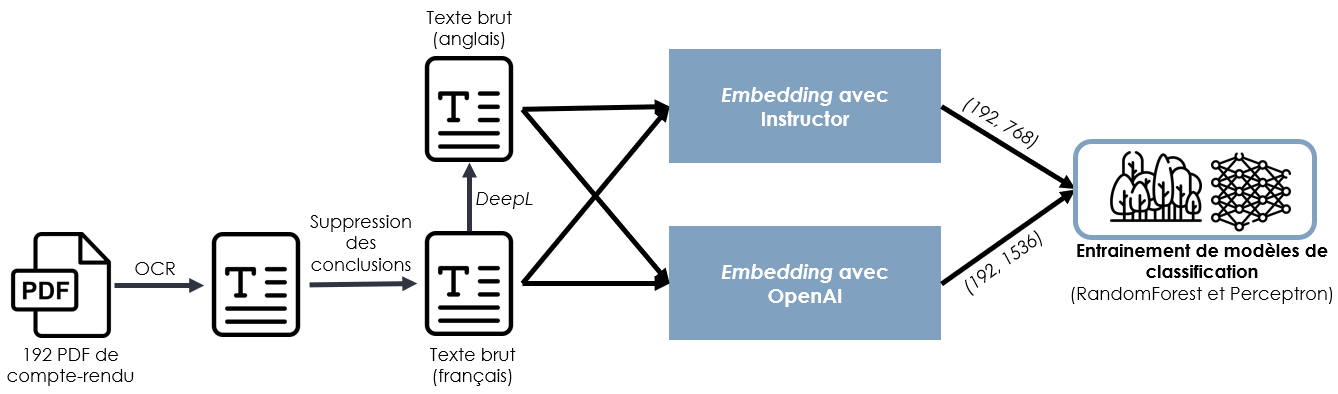
\includegraphics[width=1\textwidth]{figures/myoclassify_flow.png}
 \caption[Entraînement modèle \textit{MyoClassify}]{Étapes de préparation et d'entraînement des modèles de \textit{MyoClassify}}
 \label{fig:myoclassify_flow}
\end{figure}
\subsection{Méthodologie}
La figure \ref{fig:myoclassify_flow} représente l'ensemble des étapes réalisées pour préparer les données et entraîner un modèle de classification. Pour l'ensemble de ces rapports nous avons réalisé une étape de détection de texte par \gls{ocr} avec \textit{Tesseract}, puis nous avons retiré les conclusions des rapports (indiquant la décision de diagnostic final, c'est-à-dire le label). A partir de ces conclusions nous avons labellisé à la main chaque rapport avec un diagnostic parmi les 5 catégories listée ci-dessus.

La contenu de chaque rapports (texte brut sans la partie conclusion) a été traduit en anglais grâce à l'\gls{api} DeepL afin de comparer les performances sur les textes anglais (traduit) et français (orignaux). Puis ces textes ont été encodés numériquement grâce à deux modèles\gls{llms} d'\textit{embedding}: le modèle d'OpenAI (disponible uniquement via \gls{api}) et le modèle \textit{Instructor-Large} (auto-hébergé). Les modèles d'\textit{embedding} sont des modèles prenant en entré un texte (un mot, une phrase, un paragraphe ou un document) et qui produisent en sortie un vecteur numérique de grande taille capturant le sens sémantique du document d'entrée. Par exemple pour le modèle \textit{Instructor-Large}, le vecteur numérique de sortie pour un document possède une dimension de (1, 768). et (1, 1536) pour le modèle d'OpenAI. Ces modèles sont des boites noires, c'est à dire que la signification des centaines (voir milliers dans le cas d'OpenAI) de valeur numérique décrivant le document ne sont pas connues, cependant elles représentent le sens sémantique du texte.
A partir de ces 4 jeux de données (192 rapports dans 4 conditions: français/anglais et \textit{embedding} par OpenAI ou Instructor), nous avons entraîné et comparé les performances pour la prédiction de diagnostic de deux algorithmes: les \textit{random forest} et les perceptrons (réseaux de neurones simple). Nous avons retiré du jeu de données les 54 rapports sans diagnostic, car ils ne peuvent pas être utilisés pour l'entraînement des modèles à apprentissage supervisé ce qui aboutis à 138 rapports utilisés sur 4 labels différents pour l'entraînement des modèles (\gls{nm}, \gls{com}, \gls{cnm}, non-CM).
\begin{table}[htbp]
\centering
\caption{Nombre de rapports par diagnostic}
\label{tab:number_patients}
\begin{tabularx}{\textwidth}{|X|X|}
\hline
\textbf{Diagnostic} & \textbf{Nombre de rapports} \\
\hline
Myopathie à Némaline (NM) & 44 \\
\hline
Myopathie à Cores (COM) & 48 \\
\hline
Myopathie centronucléaire (CNM) & 16 \\
\hline
Diagnostic non établis (UNCLEAR) & 54 \\
\hline
Autre (non-CM) & 30 \\
\hline
\end{tabularx}
\end{table}

\subsection{Résultats des entraînements et performances des systèmes d'\textit{embedding}}
Au total 8 conditions expérimentales pour la prédiction de diagnostics ont été évaluées: \textit{Embedding} OpenAI vs Instructor, rapports en Français vs traduits Anglais, \textit{Random Forest} vs Perceptrons. Pour chacune des conditions expérimentales, les hyper-paramètres des modèles ont été optimisés par grille et les performances ont été évaluées grâce à 10 cross-validations. Ceci a été fait pour (i) obtenir des modèles avec les meilleures performances possible (optimisation par grille) et (ii) avoir une estimation robuste des performances (moyenne sur 10 essais par cross-validation). L'ensemble des résultats de ces entraînements (métriques de performances et modèles) sont disponibles en ligne à l'adresse: \href{https://wandb.ai/lambda-science/myo-text-classify/}{https://wandb.ai/lambda-science/myo-text-classify/}. 
\begin{table}[htbp]
\centering
\caption{Récapitulatif des performances des modèles \textit{MyoClassify}}
\label{tab:myoclassify_metrics}
\begin{tabularx}{\textwidth}{|X|X|X|X|X|X|}
\toprule
\textbf{Nom} & \textbf{Exactitude} & \textbf{Exact. Pond.} & \textbf{F1 pond.} & \textbf{F1-Macro} & \textbf{F1 classe CNM} \\\hline
Instructor FR RF & 0.6522 & 0.5556 & 0.6231 & 0.5408 & 0.1053 \\ \hline
Instructor EN RF & 0.6667 & 0.5436 & 0.6215 & 0.5172 & 0 \\ \hline
Instructor FR MLPC & 0.6739 & 0.5703 & 0.6597 & 0.5608 & 0.07692 \\ \hline
Instructor EN MLPC & 0.6449 & 0.5761 & 0.6359 & 0.5792 & 0.32 \\ \hline
Openai FR RF & 0.6087 & 0.5591 & 0.6022 & 0.5777 & 0.4545 \\ \hline
Openai EN RF & 0.6522 & 0.5792 & 0.639 & 0.5996 & 0.4 \\ \hline
Openai FR MLPC & 0.6377 & 0.6 & 0.6345 & 0.6128 & 0.5385 \\ \hline
\textbf{Openai EN MLPC} & \textbf{0.6957} &\textbf{0.6666}& \textbf{0.6931} &\textbf{ 0.68} & \textbf{0.6429} \\ \hline
\end{tabularx}
\end{table}
\begin{figure}[htbp]
 \centering
 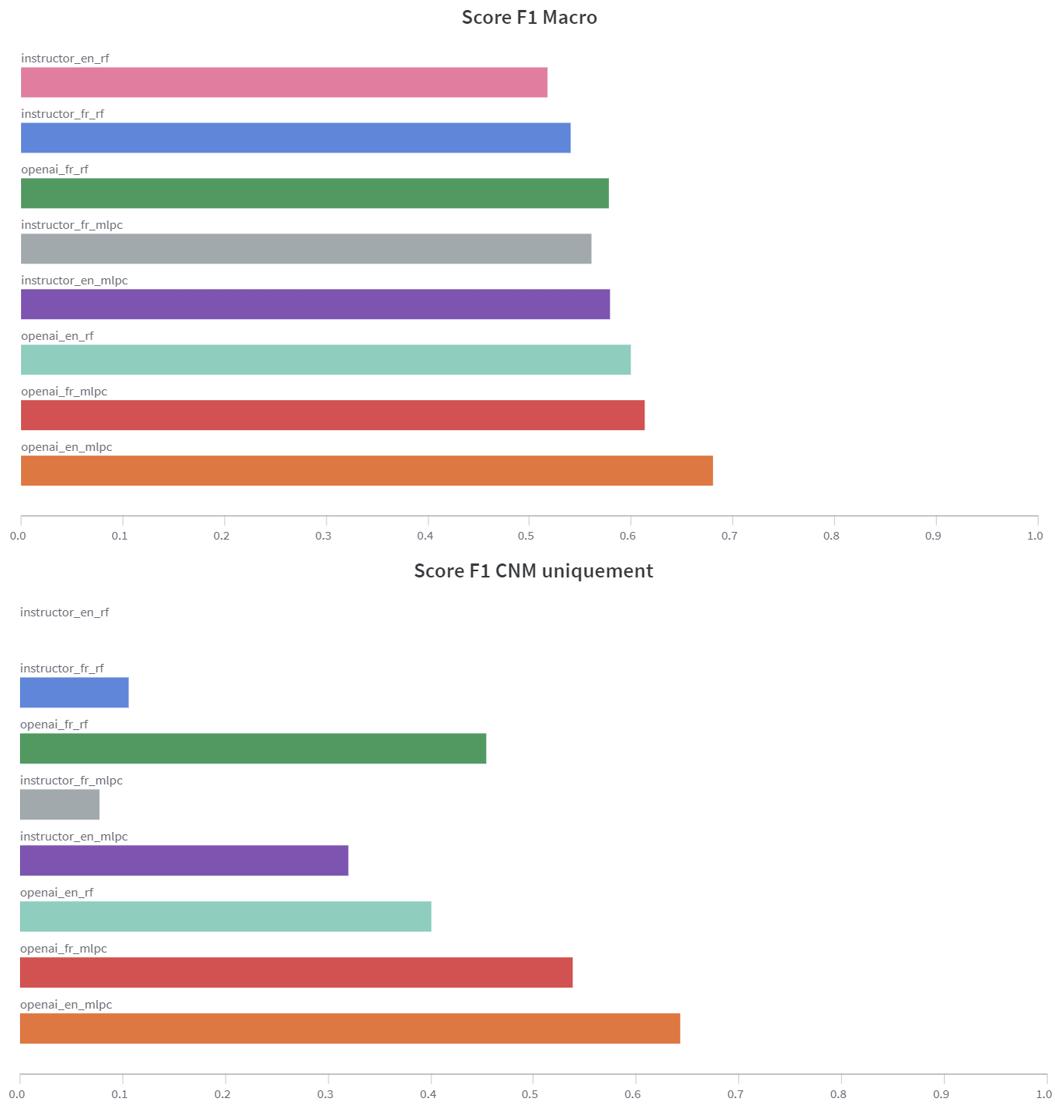
\includegraphics[width=1\textwidth]{figures/histo_myoclassify.png}
 \caption[Histogrammes des performances des modèle \textit{MyoClassify}]{Histogrammes des performances des modèles \textit{MyoClassify} pour le score F1-macro (haut) et le score F1 pour la classe minoritaire (CNM) uniquement (bas)}
 \label{fig:myoclassify_histo}
\end{figure}
\begin{figure}[htbp]
 \centering
 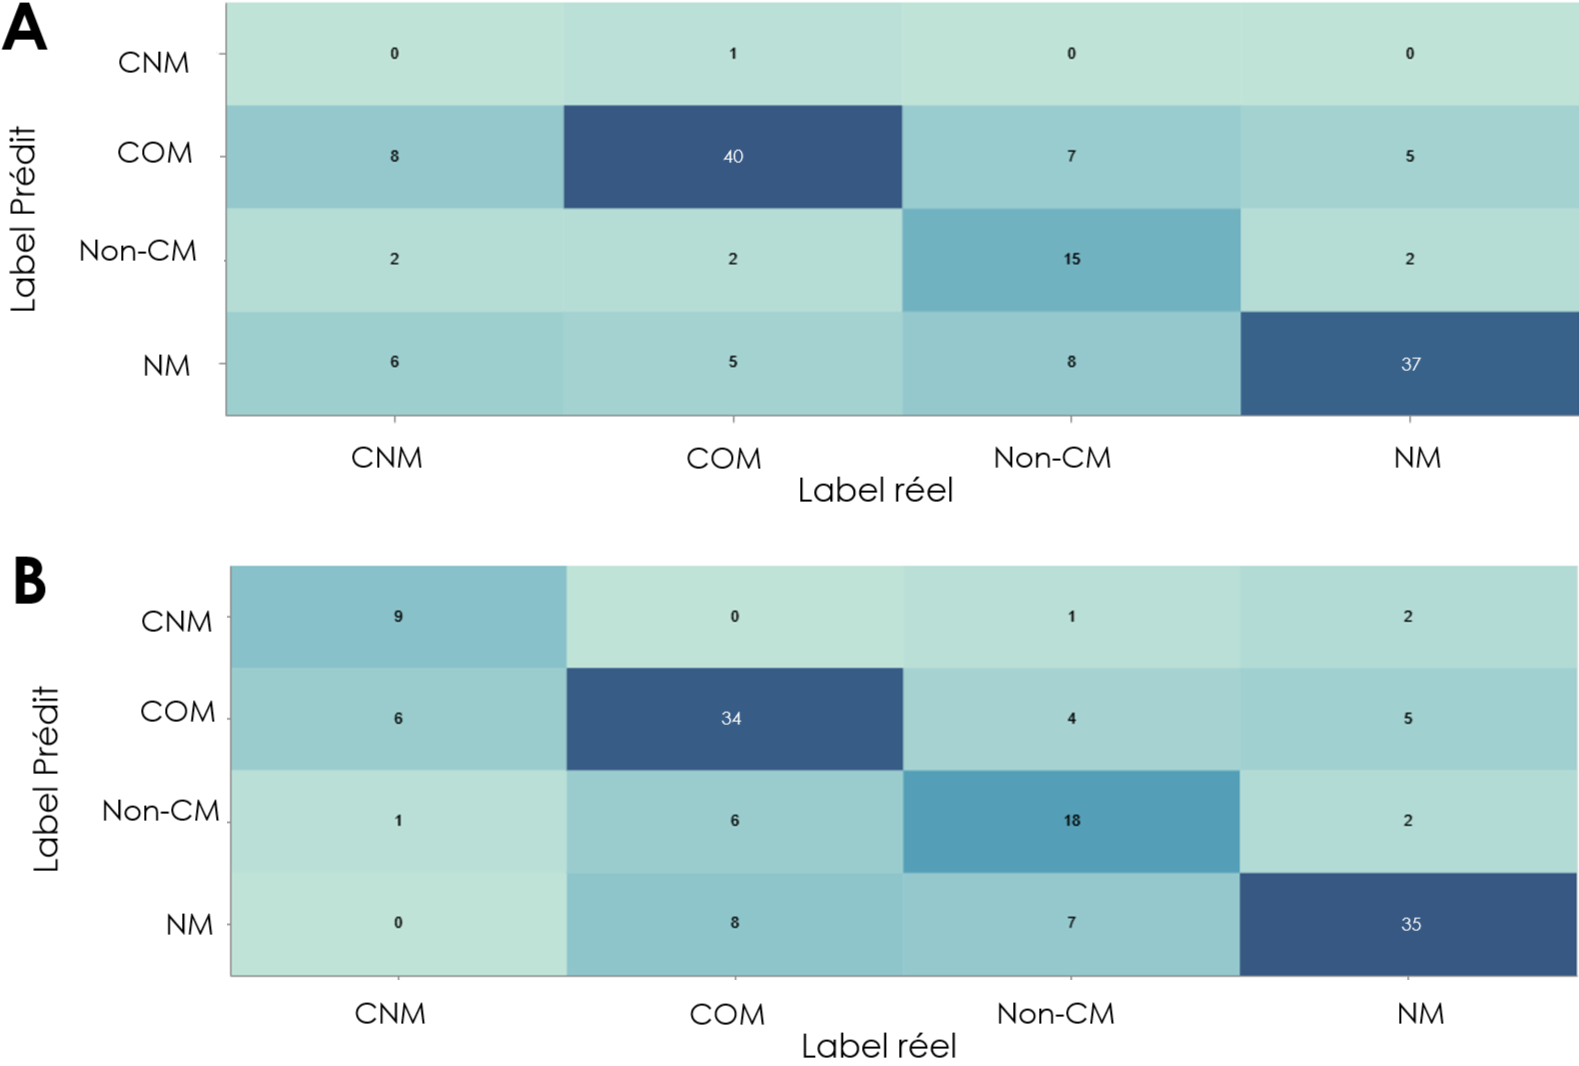
\includegraphics[width=1\textwidth]{figures/matrix_conf_myoclassify.png}
 \caption[Matrice de confusion \textit{MyoClassify}]{Matrice de confusion des modèles \textit{MyoClassify} pour le moins bon (\textit{instructor\_en\_rf} en haut) et le meilleur modèle (\textit{openai\_en\_mlpc} en bas) en terme de score F1}
 \label{fig:myoclassify_conf}
\end{figure}

Sur le tableau \ref{tab:myoclassify_metrics} et les figures \ref{fig:myoclassify_histo} et \ref{fig:myoclassify_conf} on observes que, au global, les performances à travers les conditions en terme de score F1 sont située dans un intervalle entre 0.51 et 0.68. Les modèles entraînés sur la base du modèle d'\textit{embedding} auto-hébergé \textit{Instructor} ont eu de moins bonne performances à travers toutes les conditions. Dans le cadre du modèle d'\textit{embedding} d'OpenAI, la traduction des rapports en anglais a permis d'obtenir de meilleures performances dans toutes les conditions. De même, l'utilisation d'un perceptron multi-couche a permis d'obtenir de meilleures performances en terme de score F1 dans toutes les conditions par rapport à la \textit{random forest}.

De plus, il est à noter que pour la classe minoritaire (les \gls{cnm} avec 16 rapports), les performances des modèles sont très faibles pour l'\textit{embedding} du modèle \textit{Instructor}. Par exemple, pour notre modèle \textit{Instructor\_FR\_RF}, aucune \gls{cnm} n'a été prédite (matrice de confusion \ref{fig:myoclassify_conf}). Le modèle \textit{OpenAI\_EN\_MLPC} quant à lui obtient de meilleurs performances et a été capable de prédire 9 des 16 \gls{cnm}. 

En terme de performances brutes, il semble recommandable de: (i) traduire les comptes-rendus en anglais, (ii) d'utiliser le modèle d'OpenAI pour l'\textit{embedding} et (iii) d'entrainer un perceptron multi-couche pour apprendre à différencier les diagnostics en fonction des \textit{embeddings} des rapports. 

\section{\textit{MyoSearch}: un moteur de recherche de patients}
L'\textit{embeddings} permet de représenter un texte sous forme numérique en capturant son sens sémantique. Il est alors possible de calculer un score de similarité entre une requête en texte libre et une masse de documents pour trouver le document le plus proche. Avec \textit{MyoSearch} nous avons créé un outil qui permet de faire des requêtes en texte libre parmi l'ensemble des rapports de biopsies de patients disponibles. Il est alors possible de chercher rapidement chez quels patients un symptôme ou diagnostic en particulier est présent. Cette création de moteur de recherche est totalement automatique et ne nécessite aucun travail d'annotation. Elle se déroule en deux phases: (i) l'ingestion des données pour constituer la base de données puis (ii) la phase de requêtage de la base de données en fonction de l'entrée de l'utilisateur.

\subsection{Ingestion des rapports: création de la base de données de vecteurs}
\begin{figure}[htbp]
 \centering
 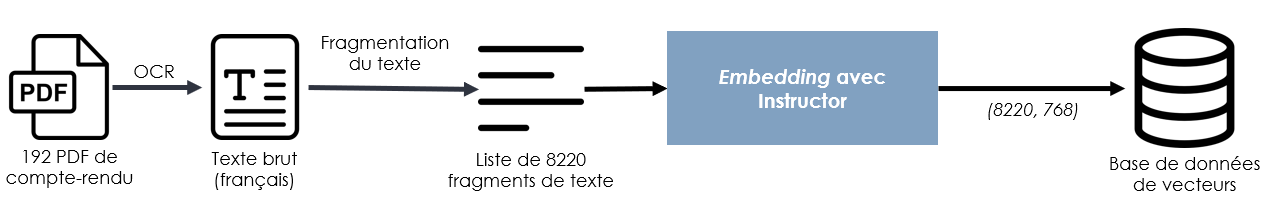
\includegraphics[width=1\textwidth]{figures/myosearch_ingest.png}
 \caption[Ingestion des données dans \textit{MyoSearch}]{Schéma de l'ingestion des données pour le moteur de recherche \textit{MyoSearch}}
 \label{fig:myosearch_ingest}
\end{figure}

A la différence de \textit{MyoClassify}, cette fois ci nous ne voulons pas générer 1 \textit{embedding} par document mais plutôt séparer les documents en fragments et avoir un \textit{embedding} par fragment de document. Nous avons choisis de découper les documents en fragments de le taille d'une phrase et ainsi d'obtenir un \textit{embedding} pour chaque phrase du document. Ceci permet d'obtenir de meilleur résultat lors du requêtage de la base de données car le sens sémantique de chaque phrase va pouvoir être comparé à la requête, plutôt que la moyenne de l'ensemble du document.

La figure \ref{fig:myosearch_ingest} présente la phase d'ingestion des données. Nous avons d'abord détecté le texte des rapports PDF par \gls{ocr}. Comme cette détection est hétérogène et bruitée, il est difficile de trouver les bornes exact des phrases. Donc nous avons fragmenter le contenu en fragment de taille de maximale de 100 \textit{tokens} (environ 30 à 50 mots) avec un recouvrement de 50. Pour 192 rapports, cela représente 8220 fragments de texte. Pour ces 8220 fragments nous avons calculé leur \textit{embedding} grâce au modèle \textit{Instructor} et nous les avons intégrés dans une base de données \textit{ChromaDB}, spécifique au stockage et requêtage de vecteur. Pour chaque fragment il est possible d'ajouter des méta-données qui peuvent servir de filtre pour les requêtes comme le diagnostic final ou le gène responsable de la maladie.

\subsection{Requêtage des données}
\begin{figure}[htbp]
 \centering
 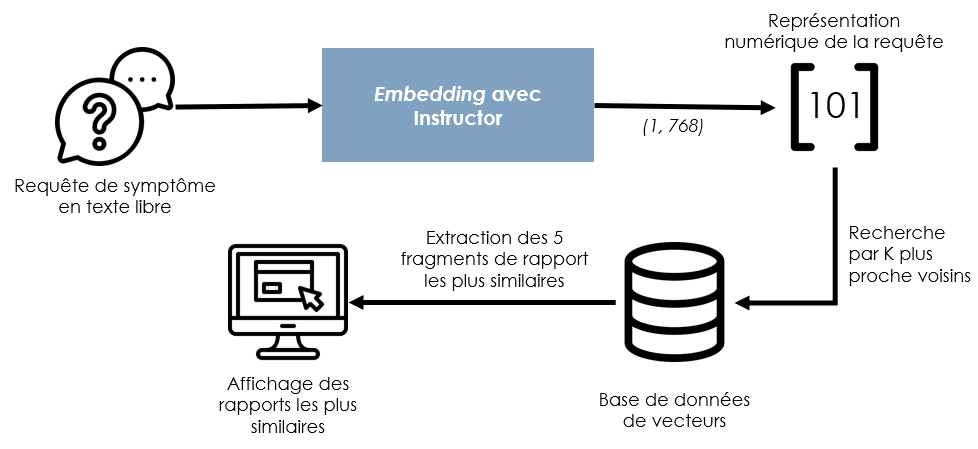
\includegraphics[width=1\textwidth]{figures/myosearch_query.png}
 \caption[Requêtage des données dans \textit{MyoSearch}]{Schéma du requêtage des données dans \textit{MyoSearch}}
 \label{fig:myosearch_query}
\end{figure}
Quand l'ensemble des documents ont été découpés et ingérés dans la base de données, il est possible de réaliser des requêtes. La figure \ref{fig:myosearch_query} présente la phase de requêtage des données. L'utilisateur peut entrer via l'interface web un symptôme d'intérêt en texte libre tel que "surcharge lipidique". Cette requête va ensuite être transformé en vecteur numérique par le modèle d'\textit{embedding }\textit{Instructor}. Ce vecteur va être comparé à la base de données de vecteur pour rechercher le top 5 plus proche voisin grâce à un algorithme nommé \textit{Hierarchical Navigable Small Worlds, HNSW}. Les cinq fragments avec les scores de similarité les plus proches sont ensuite affichés sur l'interface web. Le tableau \ref{tab:myosearch_results} présente les résultats obtenus pour une requête dans MyoSearch. Par exemple pour la requête "surcharge lipidique" les trois rapports les plus proches font mention d'une surcharge en lipides chez des patients dont (i) le diagnostic n'est pas connu, (ii) le diagnostic n'est pas une myopathie congénitale et (iii) chez un patient avec une \gls{nm}. Cette recherche est aussi multi-linguales, en effet le modèle d'\textit{embedding} étant multi-langues, la recherche entre une base de données française et une requête en anglais est possible, ou inversement.
\begin{table}[htbp]
\centering
\caption{Exemple d'une requête et des résultats de \textit{MyoSearch}}
\label{tab:myosearch_results}
\begin{tabularx}{\textwidth}{|X|X|p{1cm}|p{2cm}|}
\toprule
\textbf{Requête} & \textbf{Fragment le plus similaire} & \textbf{Rang} & \textbf{Rapport et diagnostic} \\\hline
"surcharge lipidique" & "d’inclusions. Il est à noter que l’on observe également une surcharge importante en lipides dans" \newline & 1 & 13405-105.txt UNCLEAR \\
 & "une myopathie congénitale. D'autre part, une surcharge importante en lipides qui nécessite"\newline & 2 & 11391-79.txt non-CM \\
 & "de surcharge en lipides - Technique de Koëlle : CONCLUSIONS : Anomalies caractéristiques d’une" & 3 & 5060-35.txt NM \\ \hline
\end{tabularx}
\end{table}

\section{Déploiement de l'outil}
Développé de façon \textit{open-source}, le code source de \gls{nlmyo} est disponible sur GitHub à l'adresse: \href{https://github.com/lambda-science/NLMyo}{https://github.com/lambda-science/NLMyo} soit une licence AGPL-3 assurant le statut open-source de l'outil. Une version de démonstration en ligne est déployée grâce à \textit{Streamlit} à l'adresse \href{https://lbgi.fr/NLMyo/}{https://lbgi.fr/NLMyo/}. Comme \gls{nlmyo} propose l'utilisation de \gls{llms} auto-hébergé, l'outil est hébergé sur un serveur avec un processeur 64 coeurs pour accélérer l'inférence du notre \gls{llms}. Si l'outil n'utilise que l'API OpenAI comme modèle génératif et d'\textit{embedding} alors il est possible d'héberger l'application sur un serveur avec très peu de ressource de calcul.

\section{Discussions et perspectives de développement}
\gls{nlmyo} mets à dispositions des outils permettant le traitement de façon massive de rapports de comptes-rendus médicaux et notamment des rapports de biopsie. Cependant les défis pour rendre l'outil robuste sont multiples. 

Le premier défi concerne MyoSearch, le moteur de recherche de patient. Bien que la méthode soit fonctionnelle et novatrice, il n'est actuellement possible que de chercher un symptôme à la fois. De plus les résultats obtenus ne sont pas tout le temps pertinents. Un travail d'amélioration de la méthode de fragmentation et de requêtage est nécessaire. Par exemple, il faudrait créer un système permettant de croiser les résultats des requêtes pour plusieurs symptômes, permettant ainsi de cherche un profil de symptômes complet. De plus, l'ajout de méta-données supplémentaires aux fragments (tel que les informations complètes sur les patients) permettrait de réaliser des requêtes plus fine pour ne sélectionner par exemple que les patients liée à un gène en particulier.

Le second défi majeur concerne la protection de la confidentialité des données de santé. En effet, certain outils, pour obtenir les meilleures performances, reposent sur l'utilisation de \gls{llms} externe via des l'\gls{api} OpenAI, ce qui est problématique dans le cadre de données sensibles, même anonymisées. Pour cela nous avons aussi proposé une alternative avec un modèle auto-hébergé mais pour l'instant celui-ci sous-performe. Par exemple dans \textit{MyoExtract}, les informations extraites sont incomplètes et dans \textit{MyoClassify} les scores d'exactitude et F1 sont plus faibles au global et même très faibles pour la classe minoritaire (\gls{cnm}). Cependant la recherche en terme de \gls{llms} est un domaine très dynamique et il est très probable qu'une solution auto-hébergée et performante soit disponible sous peu.